\documentclass{classrep}
\usepackage[utf8]{inputenc}
\usepackage{color}
\usepackage{graphicx} 
\usepackage{polski}
\usepackage{amsmath}
\usepackage{amsfonts}
\usepackage{amssymb}
\usepackage{lastpage}
\usepackage{indentfirst}
\usepackage{float}
\usepackage{verbatim}
\usepackage{graphicx}
\usepackage{fancyhdr}
\usepackage{listings}
\usepackage{color}
\DeclareUnicodeCharacter{00A0}{~}
\begin{titlepage}
\studycycle{Informatyka, studia dzienne, inż I st.}
\coursesemester{V}

\coursename{Sztuczna inteligencja i systemy ekspertowe}
\courseyear{2018/2019}

\courseteacher{Dr inż. Krzystof Lichy}
\coursegroup{Piątek, 9:30}

\author{
  \studentinfo{Krzysztof Barden}{210139}
}

\title{Zadanie 1: Piętnastka}
\end{titlepage}

\begin{document}
\maketitle
\newpage
\section{Cel}
Celem zadania było napisanie programu, który będzie rozwiązywał logiczną układankę zwaną piętnastką oraz zbadanie różnych metod przeszukiwania stanu.

\section{Wprowadzenie}
Piętnastka (ang. Fifteen Puzzle) to logiczna układanka składająca się z piętnastu kwadratowych klocków o jednakowych rozmiarach, numerowanych przeważnie od 1 do 15, ułożonych na planszy w kształcie kwadratu 4 na 4. Jedno miejsce na planszy pozostaje puste i umożliwia przesuwanie sąsiednich klocków względem siebie. Celem gry jest uporządkowanie klocków w kolejności rosnącej, odzwierciedlających poprawnie rozwiązany układ (rysunek 1).
Istnieją inne warianty tej układanki, w której klocków i pól może być mniej lub więcej w innych kształtach planszy (warunkiem jest możliwoć rozwiązania układanki).

\begin{figure}[h]
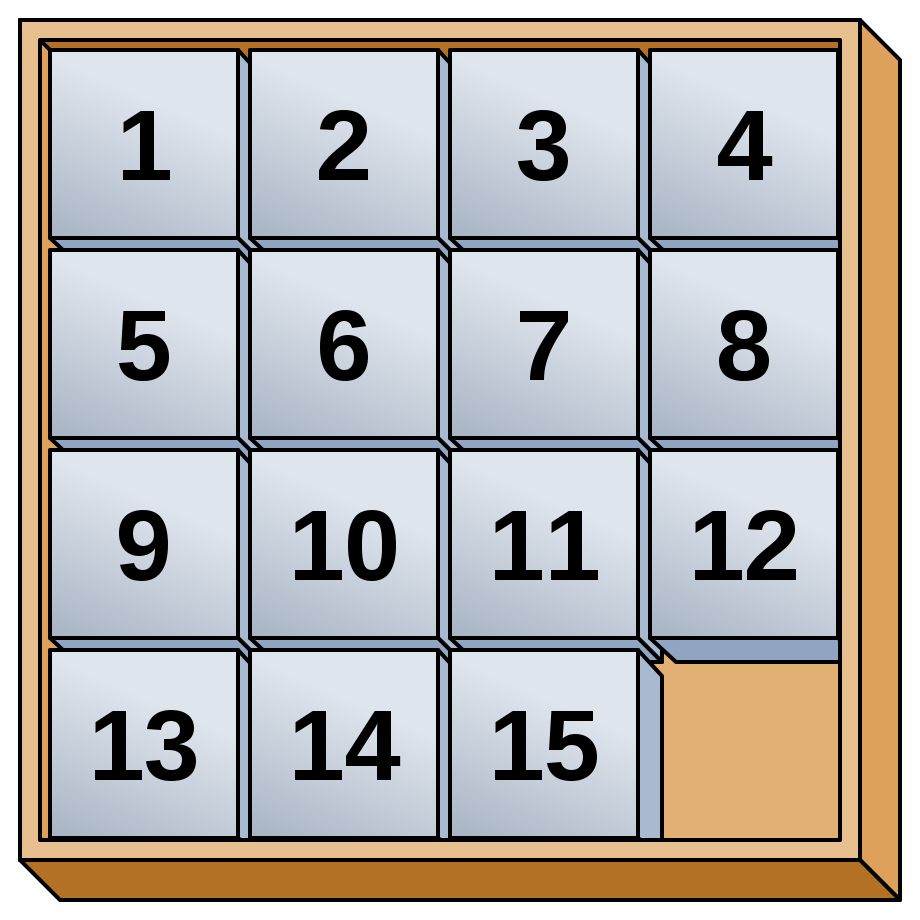
\includegraphics[width=5cm]{fifteen.jpg}
\centering
\caption{Poprawny układ piętnastki}
\end{figure}

Poszukiwanie rozwiązania łamigłówki można porównać do znajdowania ścieżki w grafie, gdzie stan układanki jest węzłem grafu, a pojedynczy ruch krawędzią. W celu odnalezienia ścieżki można zastosować różne strategie przeszukiwania przestrzeni stanów, między innymi:
\begin{itemize}
	\item BFS (breadth-first search)
	\item DFS (depth-first search)
	\item A* (A-star) z heurystykąi Manhattan, Hamminga lub innych
\end{itemize}


\subsection{BFS}
Algorytm przeszukiwania "wszerz" rozpoczyna przechodzenie grafu od zadanego wierzchołka (w tym przypadku układu startowego układanki), odwiedzając wszystkie osiągalne z niego wierzchołki na tym samym poziomie rekursji. Następnie odwiedza wszystkie osiągalne wierzchołki z wierzchołków pochodnych od poprzedniego (już na kolejnym poziomie rekursji). Z samych założeń BFS zawsze znajduje najkrótszą ścieżkę.

\subsection{DFS}
Algorytm przeszukiwania "w głąb" rozpoczyna przechodzenie grafu od zadanego wierzchołka (w tym przypadku układu startowego układanki), odwiedzając pierwszy z pochodnych wierzchołków, powtarzając to dla każdego pochodnego wierzchołka. Jeżeli algorytm nie będzie mógł wchodzić dalej, cofa się o jeden poziom rekursji i bada krawędź kolejnego nieodwiedzonego jeszcze wierzchołka.

\subsection{A*}
Algorytm heurystyczny jest to algorytmem zupełnym i optymalnym - znajduje najkrótsza ścieżkę, jeśli tylko taka istnieje. W przypadku piętnastki algorytm A* tworzy ścieżkę wybierając wierzchołek tak, aby minimalizować wartość heurestyki. Metody obliczania tej wartości to: metoda Hammminga, gdzie obliczamy ile klocków znajduje się na niewłaściwych pozycjach, metoda Manhattan, gdzie liczymy jakie odległości dzielą klocki od ich docelowych miejsc (kolumny + wiersze) i hiper-heurestyka łącząca powyższe heurestyki (suma wartosci wyliczonej z heurestyki Hamminga i heurestyki Manhattana).


\section{Opis implementacji}
Program został zaimplementowany w języku Java oraz zostały użyte dostępne na platformie WIKAMP programy i skrypty
pomagające w generowaniu i przetwarzaniu danych. Na wejściu progarm odczytuje następujące dane:
\begin{enumerate}
	\item Strategia:
	\begin{itemize}
		\item BFS (w implementacji została użyta kolejka typu FIFO (first in, first out))
		\item DFS (w implementacji została użyta kolejka typu LIFO (last in, first out), maksymalny poziom rekursji przy którym następuje nawrot został ustawiony na 20 poziom aby uniknąć zbyt długiego przeszukiwania jednej ścieżki, która i tak miałaby małą szansę na znalezienie rozwiązania)
		\item ASTR  (w implementacji tego algorytmu została użyta kolejka priorytetów ustawiana rosnąco zgodnie z wartością heurestyki)
	\end{itemize}
	
	\item Parametry wybranej strategii:
	\begin{itemize}
		\item DFS lub BFS: permutacja liter: L, R, U, D wyznaczająca ciąg ruchów poszczególnych przesunięć
		\item ASTR: heurestyka Hamminga (hamm) lub Manhattan (manh) lub własna/hiper-heurestyka (own); w celu optymalizacji w przypadku "remisów" kolejnosć ruchu jest ustalana losowo  (Las Vegas Algorithm)
	\end{itemize}
	
	\item Nazwa pliku ze stanem początkowym układanki:
	\begin{itemize}
		\item Pierwsza linia: wymiary łamigłówki
		\item Druga linia: stan łamigłówki
	\end{itemize}
	
	\item Nazwa pliku wyjściowego z rozwiązaniem układanki:
	\begin{itemize}
		\item Pierwsza linia: długość rozwiązania
		\item Druga linia: sekwencja ruchów
	\end{itemize}
	
	\item Nazwa pliku wyjściowego ze statystykami:
	\begin{itemize}
		\item Długość znalezionego rozwiązania
		\item Liczbę stanów odwiedzonych
		\item Liczbę stanów przetworzonych
		\item Maksymalną osiągniętą głębokość rekursji
		\item Czas trwania procesu obliczeniowego w milisekundach
	\end{itemize}
\end{enumerate}


\begin{figure}[H]
\centering
	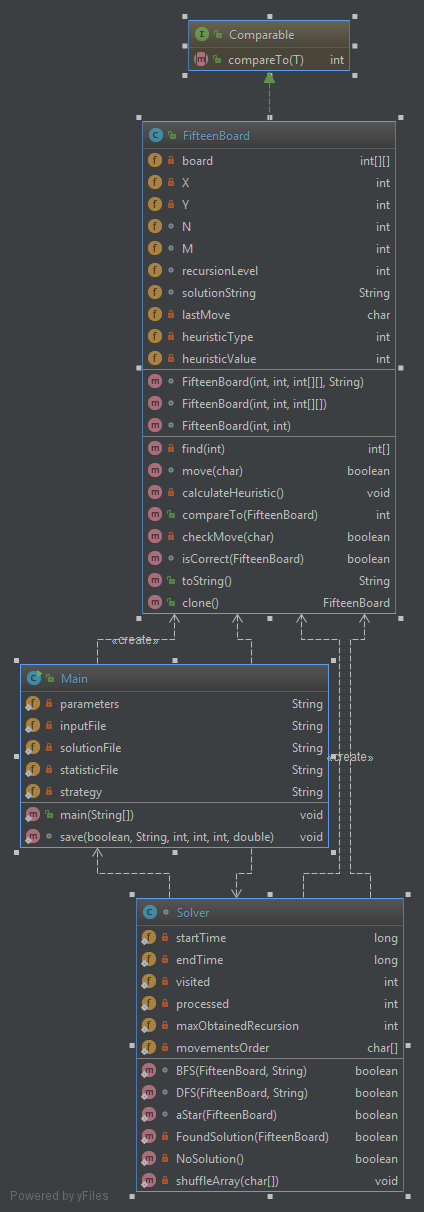
\includegraphics[height=1\textheight]{UML.png}
\caption{Diagram klas.}
\end{figure}

\section{Materiały i metody}
Za pomocą narzędzi dostępnych na platformie WIKAMP wygenerowaliśmy początkowe układy łamigłówki w odległościach 1-7. Przetestowaliśmy wyżej wymienione algorytmy w wymaganych wariantach opisanych w treści zadania korzystając z programów dostępnych na platformie WIKAMP (sprawdzanie poprawności rozwiązania). Dla przeszukiwania BFS oraz DFS skorzystaliśmy z następujących kombinacji dodatkowego parametru porządku przeszukiwania: RDLU, RDUL, DRUL, DRLU, LUDR, LURD, ULRD, ULDR. Dla przeszukiwania A*, każdy przypadek został przeprowadzony na obu heurystykach (Hamminga oraz Manhattan). Otrzymane wyniki przenieśliśmy do arkusza kalkulacyjnego, gdzie sporządziliśmy wymagane wykresy. 


\section{Wyniki}
\begin{figure}[H]
	\centering
		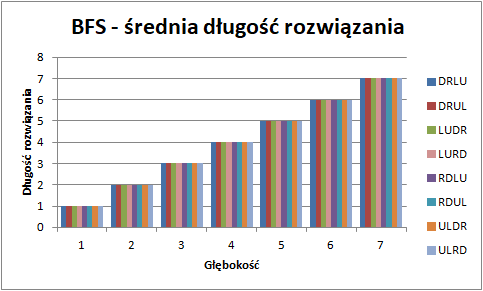
\includegraphics[width=1\textwidth]{Wykresy/1.png}
	\caption{Średnia długość rozwiązania algorytmu BFS.}
\end{figure}
\begin{figure}[H]
	\centering
		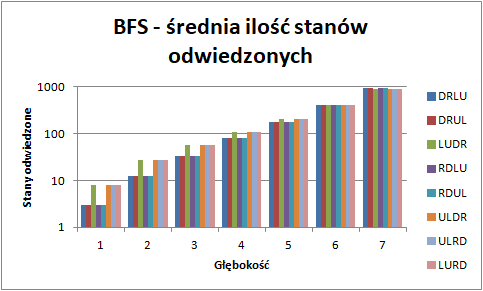
\includegraphics[width=1\textwidth]{Wykresy/2.png}
	\caption{Średnia ilość stanów odwiedzonych algorytmu BFS.}
\end{figure}
\begin{figure}[H]
	\centering
		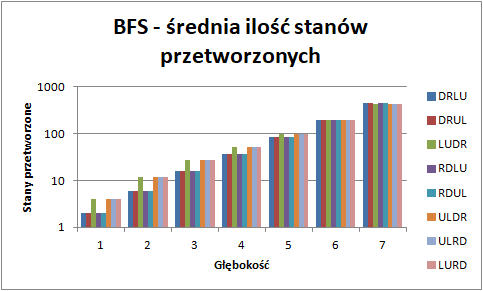
\includegraphics[width=1\textwidth]{Wykresy/3.png}
	\caption{Średnia ilość stanów przetworzonych algorytmu BFS.}
\end{figure}
\begin{figure}[H]
	\centering
		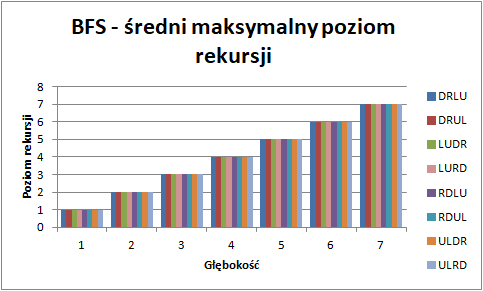
\includegraphics[width=1\textwidth]{Wykresy/4.png}
	\caption{Średnia maksymalna rekursja algorytmu BFS.}
\end{figure}
\begin{figure}[H]
	\centering
		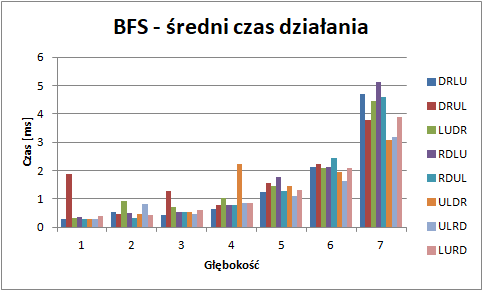
\includegraphics[width=1\textwidth]{Wykresy/5.png}
	\caption{Średni czas działania algorytmu BFS.}
\end{figure}
\begin{figure}[H]
	\centering
		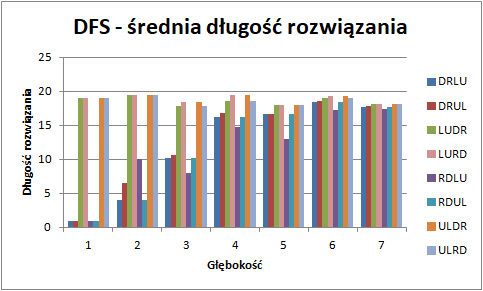
\includegraphics[width=1\textwidth]{Wykresy/6.png}
	\caption{Średnia długość rozwiązania algorytmu DFS.}
\end{figure}
\begin{figure}[H]
	\centering
		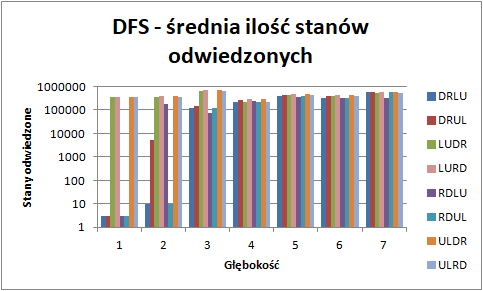
\includegraphics[width=1\textwidth]{Wykresy/7.png}
	\caption{Średnia ilość stanów odwiedzonych algorytmu DFS.}
\end{figure}
\begin{figure}[H]
	\centering
		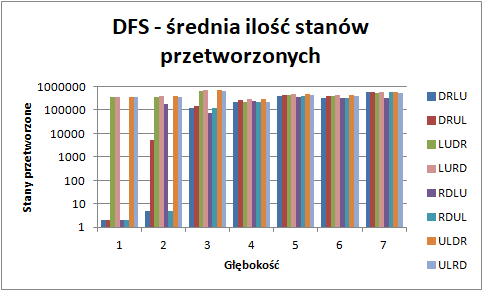
\includegraphics[width=1\textwidth]{Wykresy/8.png}
	\caption{Średnia ilość stanów przetworzonych algorytmu DFS.}
\end{figure}
\begin{figure}[H]
	\centering
		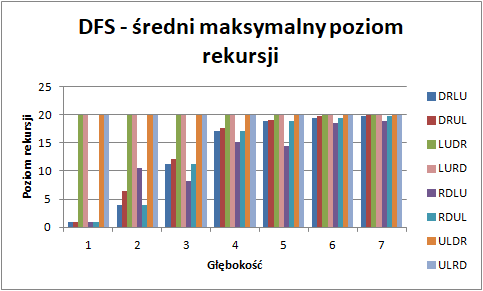
\includegraphics[width=1\textwidth]{Wykresy/9.png}
	\caption{Średnia maksymalna rekursja algorytmu DFS.}
\end{figure}
\begin{figure}[H]
	\centering
		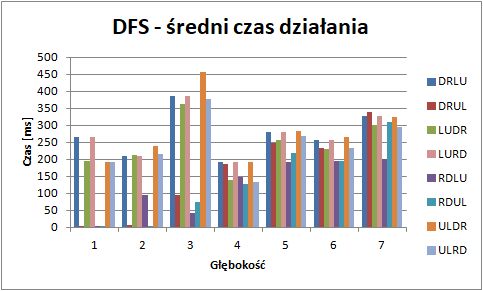
\includegraphics[width=1\textwidth]{Wykresy/10.png}
	\caption{Średni czas działania algorytmu DFS.}
\end{figure}
\begin{figure}[H]
	\centering
		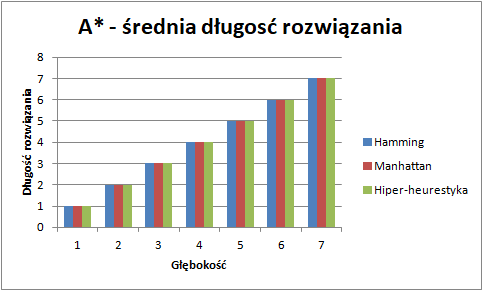
\includegraphics[width=1\textwidth]{Wykresy/11.png}
	\caption{Średnia długość rozwiązania algorytmu A*.}
\end{figure}
\begin{figure}[H]
	\centering
		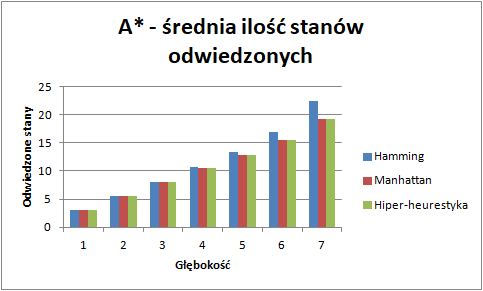
\includegraphics[width=1\textwidth]{Wykresy/12.png}
	\caption{Średnia ilość odwiedzonych stanów algorytmu A*.}
\end{figure}
\begin{figure}[H]
	\centering
		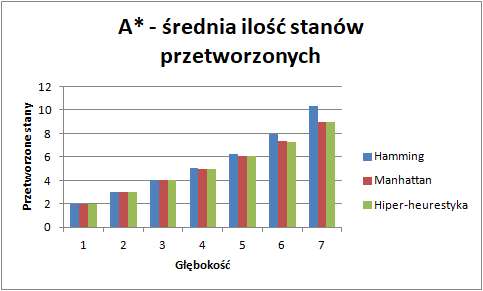
\includegraphics[width=1\textwidth]{Wykresy/13.png}
	\caption{Średnia ilość przetworzonych stanów algorytmu A*.}
\end{figure}
\begin{figure}[H]
	\centering
		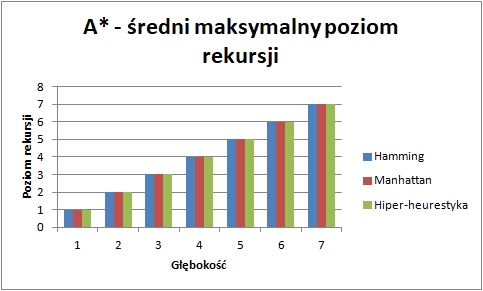
\includegraphics[width=1\textwidth]{Wykresy/14.png}
	\caption{Średnia maksymalna rekursja algorytmu A*.}
\end{figure}
\begin{figure}[H]
	\centering
		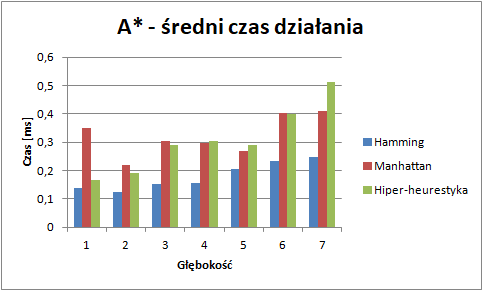
\includegraphics[width=1\textwidth]{Wykresy/15.png}
	\caption{Średni czas działania A*.}
\end{figure}
\begin{figure}[H]
	\centering
		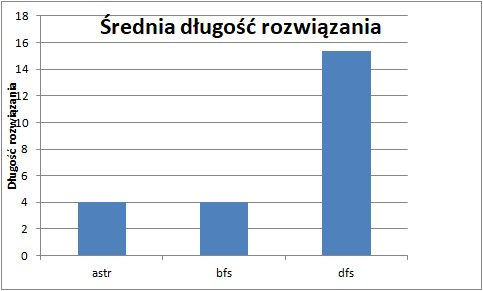
\includegraphics[width=1\textwidth]{Wykresy/16.jpg}
	\caption{Średnia długość rozwiązania wszystkich algorytmów.}
\end{figure}
\begin{figure}[H]
	\centering
		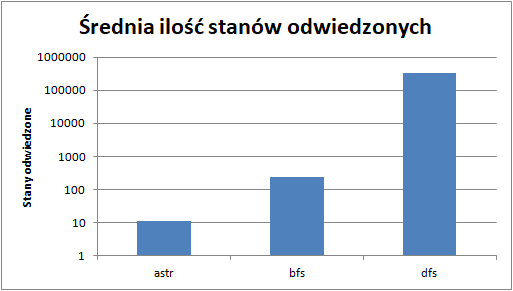
\includegraphics[width=1\textwidth]{Wykresy/17.png}
	\caption{Średnia ilość odwiedzonych stanów wszystkich algorytmów.}
\end{figure}
\begin{figure}[H]
	\centering
		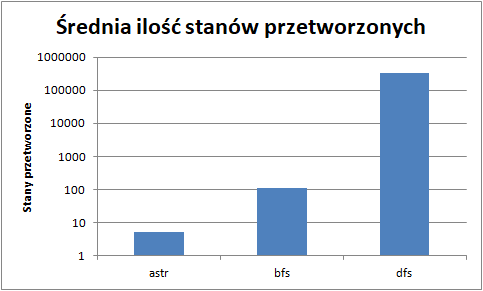
\includegraphics[width=1\textwidth]{Wykresy/18.png}
	\caption{Średnia ilość przetworzonych stanów wszystkich algorytmów.}
\end{figure}
\begin{figure}[H]
	\centering
		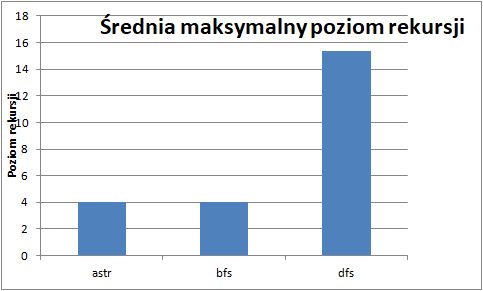
\includegraphics[width=1\textwidth]{Wykresy/19.png}
	\caption{Średnia maksymalna rekursja wszystkich algorytmów.}
\end{figure}
\begin{figure}[H]
	\centering
		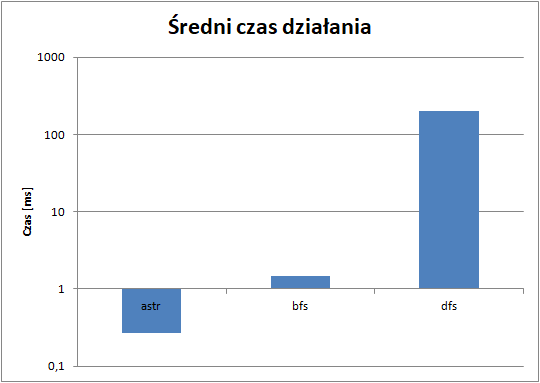
\includegraphics[width=1\textwidth]{Wykresy/20.png}
	\caption{Średniczas działania wszystkich algorytmów.}
\end{figure}

\section{Dyskusja}
\subsection{Średnia długość rozwiązania}
Algorytmy BFS oraz A*  zwracają rozwiązania o takiej samej długości co głębokość układanki - z samych założeń znajdują one najkrótsze rozwiązania.

Algorytm DFS rzadko znajduje najkrótsze rozwiązania. Jest to uzależnione od kolejności rozpatrywania ruchów. Niekorzystny układ ruchów może spowodować długie rozwiązania nawet przy układach o małej głębokosci (aż do 20 ruchów). Wraz ze wzrostem głębokości (a więc też ilości istniejących krawędzi w grafie) prawodobieństwo na znalezienie najkrótszego rozwiązania drastycznie maleją. 
\subsection{Średnia ilość odwiedzonych stanów}
Ilość odwiedzonych stanów dla algorytmu A* jest najmniejsza ze wszystkich użytych algorytmów. Heurestyka Mahattana i hiper-heurestyka mają podobne wyniki i są lepsze niż heurestyka Hamminga. Wartości nie przekraczają 46. 

Dla algorytmu BFS, wraz ze wzrostem głębokości wartości szybko rosną osiągając prawie 1000 odwiedzonych stanów.

Dla algorytmu DFS głębokość nie ma największego znaczenia. Najbardziej wpływa kolejność wykonywanych ruchów. Dla małych głebokości jest to najlepiej widoczne. 
\subsection{Średnia ilość przetworzonych stanów}
Algorytm A* średnio odwiedza mniej niż 10 stanów w celu znalezienia rozwiązania (dla głębokości 7 herurestyka Hamminga potrzebuje średnio ok 10 przetworzonych stanów, zaś Manhattan i hiper-heurestyka niecałe 9).

Ilość przetworzonych stanów dla algorytmu BFS wynosi ok. połowe stanów odwiedzonych jednak nadal jest to więcej niż w przypadku A*.
DFS przetwarza on ponad 99\% odwiedzonych przez siebie rozwiązań, pokazując nieprzydatność do rozwiązywania tej układanki. 
\subsection{Średni maksymalny poziom rekursji}
Zgodnie z definicją BFS i A* nie maksymalny poziom rekursji nie przekracza głębokości rozwiązania.

W przypadku algorytmu DFS zadany maksymalny poziom rekursji jest prawie zawsze osiągany co pokazuje słuszność użycia tego limitu. 
\subsection{Średni czas działania}
Na czas działania algorytmu wpływają różne czynniki takie jak programy pracujące w tle lub sposób przydzielania przez system zasobów dla programu co wpływa na zakłócenia w pomiarach.
Ilość odwiedzonych i przetworzonych stanów odzwierciedla się w czasie działania co powoduje że algorytm A* jest najszybszy. 
Jednak większy wpływ w przypadku tego algorytmu mają sposoby obliczania heurestyki. Sprawdzenie czy dany klocek w układance jest na swoim miejscu (Hamming) jest o wiele mniej kosztowne od liczenia odległości dla każdego klocka (Manhattan). Hiper-heurestyka jest zestawieniem obu tych heurestyk więc w teorii powinna zajmować najwięcej czasu na obliczenie. 
 
Czas rozwiązywania za pomocą algorytmu BFS potrafi być zróżnicowany ze względu na możliwość przyjęcia różnych strategi przeszukiwania stanów. Korzystne kombinacje kroków dla większych głębokości są widoczne w lepszych czasach. 

Średni czas działania algorytmu DFS jest ok 200 razy większy od czasu BFS, co pokazuje dużą słabość tego algorytmu przy rozwiązywaniu tej układanki.
\subsection{Heurestyki}
W wynikach widoczne jest podobieństwo hiper-heurestyki do heurestyki Manhattana. Spowodowane jest to tym, że sumy odległości są o wiele większe od ilości klocków nie na swoim miejscu. 
Widać też małe różnice w skuteczności heurestyk pomiędzy małymi a większymi głębokościami układanki.

\section{Wnioski}
\begin{itemize}
	\item Algorytm A* najlepiej nadaje się do rozwiązywania "piętnastki" bez względu na wybraną heurestykę.
	\item Heurystyka Manhattana nadaję się do bardziej skomplikowanych ułożeń, a Hamminga do prostszych.
	\item Odpowiednie proporcje przy sumowaniu heurestyk w hiper-heurestyce mogłoby dać większe efekty.
	\item Algorytm BFS nie jest najbardziej optymalnym algorytmem do rozwiązywania tej układanki ale jego wyniki są zadowalające.
	\item Algorytm DFS nie jest odpowiedni do rozwiązywania "piętnastki" ze względu na zbyt długi czas działania, przypadkowość w znajdywaniu krótszych rozwiązań i zbyt duże pochłanianie zasobów programu.
\end{itemize}

\begin{thebibliography}{0}
 	\bibitem{l2short} http://www.math.edu.pl/pietnastka
 	\bibitem{l2short} https://pl.wikipedia.org/wiki/Piętnastka\_(układanka)
  	\bibitem{l2short} http://jamie-wong.com/2011/10/16/fifteen-puzzle-algorithm/
	\bibitem{l2short} https://en.wikipedia.org/wiki/Hyper-heuristic
  	\bibitem{l2short} https://pl.wikipedia.org/wiki/Algorytm\_A*
	\bibitem{l2short} https://pl.wikipedia.org/wiki/Odległość\_Hamminga
	\bibitem{l2short} https://en.wikipedia.org/wiki/Las\_Vegas\_algorithm

\end{thebibliography}


\end{document}
